
The binomial distribution is given by:
\begin{equation}
\pr{X=k}=\comb{n}{k}\times p^k\times q^{n-k}
\end{equation}
We are given $n=11$, $p=\frac{1}{3}$ and hence $q=\frac{2}{3}$
\begin{align}
\pr{X = k}={\comb{11}{k}}\brak{\frac{2}{3}}^{11-k}\brak{\frac{1}{3}}^{k}
\end{align}
%To maximise $\pr{X = k}$,
\begin{align}
%\pr{X = k}&\geq\pr{X = k+1}\\
\frac{\pr{X = k}}{\pr{X = k+1}} &\geq1
\\
\implies \frac{{\comb{11}{k}}\brak{\frac{2}{3}}^{11-k}\brak{\frac{1}{3}}^{k}}{{\comb{11}{k+1}}\brak{\frac{2}{3}}^{10-k}\brak{\frac{1}{3}}^{k+1}}&\geq1
\\
\text{or, }k&\geq3
\label{binom/2/condition1}
\end{align}
after some algebra.  Similarly, 
\begin{align}
%\frac{2(k+1)}{11-k}&\geq1\\
%\pr{X = k}&\geq\pr{X = k-1}\\
\frac{\pr{X = k}}{\pr{X = k-1}}& \geq 1\\
% \implies \frac{12-k}{2k}&\geq1\\
% &=\frac{{\comb{11}{k}}\brak{\frac{2}{3}}^{11-k}\brak{\frac{1}{3}}^{k}}{{\comb{11}{k-1}}\brak{\frac{2}{3}}^{12-k}\brak{\frac{1}{3}}^{k-1}}
k&\leq4\label{binom/2/condition2}
\end{align}
From \eqref{binom/2/condition1} and \eqref{binom/2/condition2},  it is obvious that $\pr{X = k}$ is maximized for $k=3$, $k=4$. Hence, options 2 and 3 are correct.  See Fig. 
\ref{binom/2/fig:binom dist} for a graphical verification.
%\renewcommand{\thefigure}{1}
\begin{figure}[!htb]
\centering
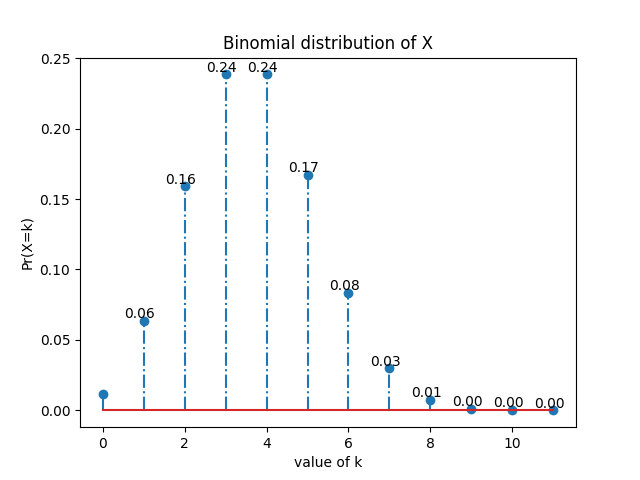
\includegraphics[width=\columnwidth]{binomial/solutions/2/Binomial-stemplot.png}
\caption{Binomial Distribution of  $X$}
\label{binom/2/fig:binom dist}
\end{figure}

